% DoD DevSecOps Software Design Document Template
% CTAS-7 / SX9 Platform
% Aligned with DoDI 5000.87 and NIST SP 800-160

\documentclass[11pt,letterpaper]{article}
\usepackage[utf8]{inputenc}
\usepackage{geometry}
\usepackage{graphicx}
\usepackage{hyperref}
\usepackage{listings}
\usepackage{xcolor}
\usepackage{fancyhdr}
\usepackage{titlesec}
\usepackage{natbib}
\usepackage{longtable}
\usepackage{tikz}
\usetikzlibrary{shapes,arrows,positioning}

\geometry{margin=1in}
\pagestyle{fancy}
\fancyhf{}
\rhead{SOFTWARE DESIGN DOCUMENT}
\lhead{\leftmark}
\rfoot{Page \thepage}
\lfoot{UNCLASSIFIED // FOUO}

% Define colors
\definecolor{dodblue}{RGB}{0,51,102}
\definecolor{codegray}{RGB}{240,240,240}

% Title formatting
\titleformat{\section}{\Large\bfseries\color{dodblue}}{\thesection}{1em}{}
\titleformat{\subsection}{\large\bfseries}{\thesubsection}{1em}{}

% Code listing style
\lstset{
    basicstyle=\ttfamily\footnotesize,
    breaklines=true,
    frame=single,
    backgroundcolor=\color{codegray},
    keywordstyle=\color{blue},
    commentstyle=\color{green!50!black},
    stringstyle=\color{orange}
}

\begin{document}

% ═══════════════════════════════════════════════════════════════════════════
% TITLE PAGE
% ═══════════════════════════════════════════════════════════════════════════

\begin{titlepage}
\centering
\vspace*{2cm}

{\Huge\bfseries\color{dodblue} Software Design Document}\\[0.5cm]
{\Large\bfseries System/Subsystem Name}\\[1cm]

\rule{\textwidth}{1.5pt}\\[0.5cm]

{\large
\begin{tabular}{ll}
\textbf{Document ID:} & SDD-XXXX-001 \\
\textbf{Version:} & 1.0 \\
\textbf{Date:} & \today \\
\textbf{Classification:} & UNCLASSIFIED // FOUO \\
\textbf{Contract:} & Contract Number \\
\textbf{CDRL:} & A-XXX \\
\end{tabular}
}

\vfill

{\large Prepared for:}\\
\textbf{Department of Defense}\\
Program Executive Office\\[1cm]

{\large Prepared by:}\\
\textbf{Organization Name}\\
Address\\[2cm]

\end{titlepage}

% ═══════════════════════════════════════════════════════════════════════════
% REVISION HISTORY
% ═══════════════════════════════════════════════════════════════════════════

\section*{Revision History}
\begin{longtable}{|p{1.5cm}|p{2.5cm}|p{3cm}|p{7cm}|}
\hline
\textbf{Version} & \textbf{Date} & \textbf{Author} & \textbf{Description} \\
\hline
1.0 & \today & Author Name & Initial Release \\
\hline
\end{longtable}

\tableofcontents
\newpage

% ═══════════════════════════════════════════════════════════════════════════
% 1. INTRODUCTION
% ═══════════════════════════════════════════════════════════════════════════

\section{Introduction}

\subsection{Purpose}
This Software Design Document (SDD) describes the software architecture and detailed design for [System Name]. This document is prepared in accordance with DoDI 5000.87 (Operation of the Software Acquisition Pathway) and NIST SP 800-160 (Systems Security Engineering).

\subsection{Scope}
[Define the scope of the software covered by this SDD]

\subsection{Applicable Documents}
\begin{itemize}
    \item RFC-9000: Synaptix9 Agnostic Core \& Ontology
    \item RFC-9001: Trivariate Hashing Standard
    \item RFC-9004: Deterministic Routing Architecture
    \item NIST SP 800-53: Security and Privacy Controls
    \item DoD Cloud Computing SRG
\end{itemize}

\subsection{Definitions and Acronyms}
\begin{longtable}{|p{3cm}|p{10cm}|}
\hline
\textbf{Term} & \textbf{Definition} \\
\hline
ATLAS & Autonomous Tactical Logic and Sensing - 1ms cognitive tick \\
\hline
SCH & Semantic Content Hash - Trivariate addressing \\
\hline
Neural Mux & Sub-250ns routing layer \\
\hline
OODA & Observe-Orient-Decide-Act loop \\
\hline
\end{longtable}

% ═══════════════════════════════════════════════════════════════════════════
% 2. SYSTEM OVERVIEW
% ═══════════════════════════════════════════════════════════════════════════

\section{System Overview}

\subsection{System Context}
[Describe the system context and external interfaces]

\subsection{System Functions}
[List and describe major system functions]

\subsection{User Characteristics}
[Describe the intended users of the system]

% ═══════════════════════════════════════════════════════════════════════════
% 3. DESIGN CONSIDERATIONS
% ═══════════════════════════════════════════════════════════════════════════

\section{Design Considerations}

\subsection{Goals and Guidelines}
\begin{itemize}
    \item RFC-9001 Compliance: All addressing uses Murmur3-128 trivariate hashing
    \item NVNN Comment Standard: Comments every 20 lines
    \item Zero-Trust Architecture: All connections authenticated
    \item DevSecOps Integration: Continuous security validation
\end{itemize}

\subsection{Development Methods}
\begin{itemize}
    \item Rust for performance-critical components
    \item Foundation crate dependencies (ctas7-foundation-*)
    \item Automated QA via ABE Lightning system
\end{itemize}

\subsection{Architectural Strategies}
[Describe key architectural decisions]

% ═══════════════════════════════════════════════════════════════════════════
% 4. ARCHITECTURAL DESIGN
% ═══════════════════════════════════════════════════════════════════════════

\section{Architectural Design}

\subsection{System Architecture}

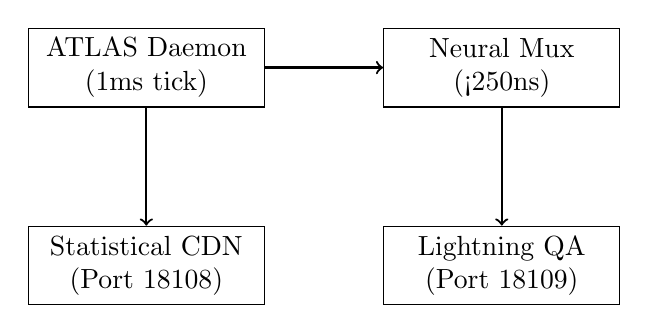
\begin{tikzpicture}[
    node distance=1.5cm,
    box/.style={rectangle, draw, minimum width=3cm, minimum height=1cm, align=center},
    arrow/.style={->, thick}
]
% Add architecture diagram here
\node[box] (atlas) {ATLAS Daemon\\(1ms tick)};
\node[box, right=of atlas] (mux) {Neural Mux\\(<250ns)};
\node[box, below=of atlas] (cdn) {Statistical CDN\\(Port 18108)};
\node[box, below=of mux] (qa) {Lightning QA\\(Port 18109)};

\draw[arrow] (atlas) -- (mux);
\draw[arrow] (atlas) -- (cdn);
\draw[arrow] (mux) -- (qa);
\end{tikzpicture}

\subsection{Component Descriptions}
[Describe each major component]

\subsection{Port Allocations (RFC-9004)}
\begin{longtable}{|l|l|l|}
\hline
\textbf{Port} & \textbf{Service} & \textbf{Description} \\
\hline
18103 & Port Manager & Dynamic port allocation \\
18108 & Statistical CDN & Content distribution \\
18109 & ABE Lightning QA & Fast static analysis \\
18110 & Zencoder Expert QA & AI-driven analysis \\
\hline
\end{longtable}

% ═══════════════════════════════════════════════════════════════════════════
% 5. SECURITY DESIGN
% ═══════════════════════════════════════════════════════════════════════════

\section{Security Design}

\subsection{Security Architecture}
Aligned with RFC-9006 (Secure Transport Profiles) and NIST SP 800-53.

\subsection{Authentication}
\begin{itemize}
    \item Zero-trust: All connections require authentication
    \item Trivariate hash-based identity verification
    \item Capability-based access control
\end{itemize}

\subsection{Encryption}
\begin{itemize}
    \item TLS 1.3 for all network communications
    \item AES-256-GCM for data at rest
    \item Key rotation per RFC-9009
\end{itemize}

\subsection{Security Controls Mapping}
\begin{longtable}{|l|p{8cm}|}
\hline
\textbf{NIST Control} & \textbf{Implementation} \\
\hline
AC-2 & Account management via ATLAS \\
AU-2 & Audit logging to Statistical CDN \\
IA-2 & Multi-factor via biometric honeypot (RFC-9007) \\
SC-8 & Transport encryption (TLS 1.3) \\
\hline
\end{longtable}

% ═══════════════════════════════════════════════════════════════════════════
% 6. DATA DESIGN
% ═══════════════════════════════════════════════════════════════════════════

\section{Data Design}

\subsection{Data Model}
[Describe the data model aligned with RFC-9005]

\subsection{Schema Specification}
All data follows RFC-9005 Unified Schema:
\begin{lstlisting}[language=json]
{
  "entity_id": "SCH:0x1234:0x01:...",
  "metadata": {
    "created": "2025-11-28T00:00:00Z",
    "version": "7.3.1"
  },
  "payload": { ... }
}
\end{lstlisting}

% ═══════════════════════════════════════════════════════════════════════════
% REFERENCES
% ═══════════════════════════════════════════════════════════════════════════

\newpage
\bibliographystyle{ieeetr}
\bibliography{references}

% ═══════════════════════════════════════════════════════════════════════════
% APPENDICES
% ═══════════════════════════════════════════════════════════════════════════

\appendix

\section{RFC Compliance Matrix}
\begin{longtable}{|l|l|l|}
\hline
\textbf{RFC} & \textbf{Requirement} & \textbf{Status} \\
\hline
RFC-9001 & Murmur3-128 trivariate hashing & Compliant \\
RFC-9002 & Unicode routing & Compliant \\
RFC-9004 & Port 18000-19000 range & Compliant \\
RFC-9005 & Unified schema & Compliant \\
\hline
\end{longtable}

\end{document}
